\subsubsection*{四、设计题}
\setcounter{problemname}{0}

\begin{problem}
指出下面的对话框设计中存在的问题,并给出改进建议。
\begin{figure}[H]
    \vspace{-0.5em}
	\centering
	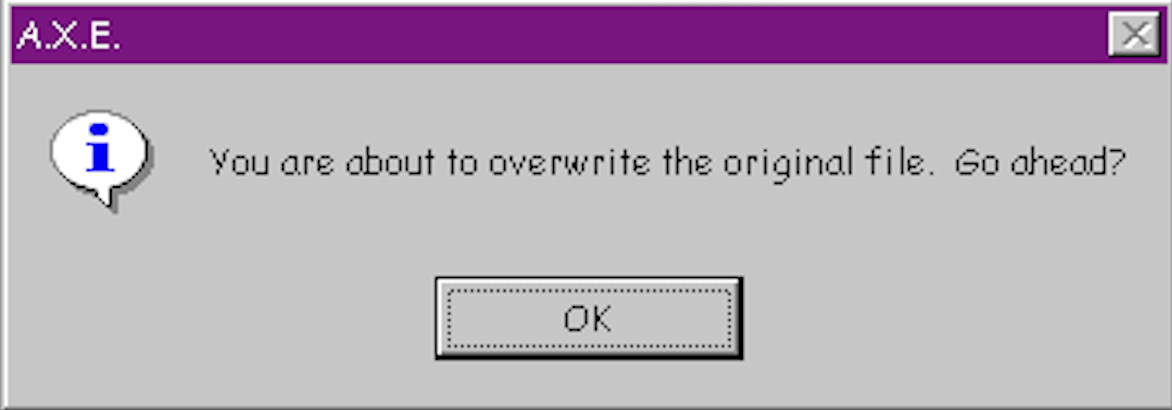
\includegraphics[width=0.5\textwidth]{1.png}
    \vspace{-1em}
\end{figure}
\end{problem}

\begin{solution}
没有讲overwrite的后果;标题A.X.E.是什么意思;只有OK,没有退出机制;
\end{solution}



\begin{problem}
人物角色是交互设计中非常重要的一项技术,能够帮助设计团队做很多设计决策。如下是某团队为某项目构造的人物角色的例子,请分析其中存在的问题,并说明什么是人物角色,以及在构建人物角色时需要注意哪些问题。
\begin{figure}[H]
    \vspace{-0.5em}
	\centering
	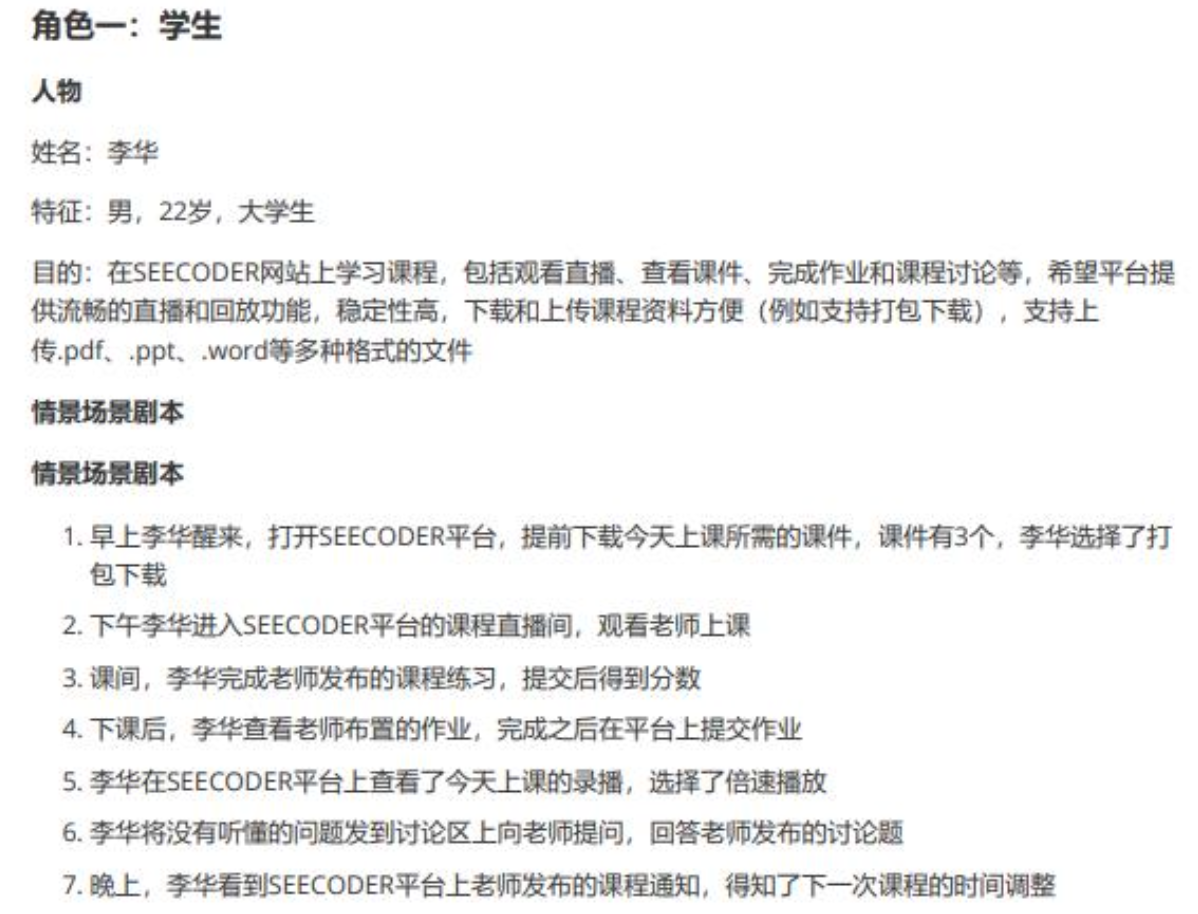
\includegraphics[width=0.7\textwidth]{2.png}
    \vspace{-1em}
\end{figure}
\end{problem}

\begin{solution}
问题:
\begin{enumerate}[label=\arabic*.]
    \item 人物信息构造不完整(没有照片);
    \item 目标不对,目标不是功能(帮助他更好的完成课程学习);
    \item 场景剧本有问题(不能写成使用手册,应该描述需求,不要使用术语,要使用自然语言);
\end{enumerate}

人物角色是基于观察到的那些真实人的行为和动机,并且在整个设计过程中代表真实的人;是在人口统计学调查收集到的实际用户的行为数据的基础上形成的综合原型。

要注意那些与软件用户界面设计有关的角色特征;要关注使角色之间彼此相区别的特征;要留心焦点角色 (最常见、最典型的角色)。
\end{solution}



\begin{problem}
作为组织者组织一次会议是一项非常繁琐的工作,涉及到很多细节事务。在用户体验设计中,层次化任务分析用来分析并描述用户如何为达到目标所进行的一系列任务,以及用户与软件系统是如何交互的。如果你将\textbf{组织一次会议},请使用层次化任务分析技术完成会议组织的层次化任务分析的文字和图形描述。
\end{problem}

\begin{solution}
\begin{figure}[H]
    \vspace{-0.5em}
	\centering
	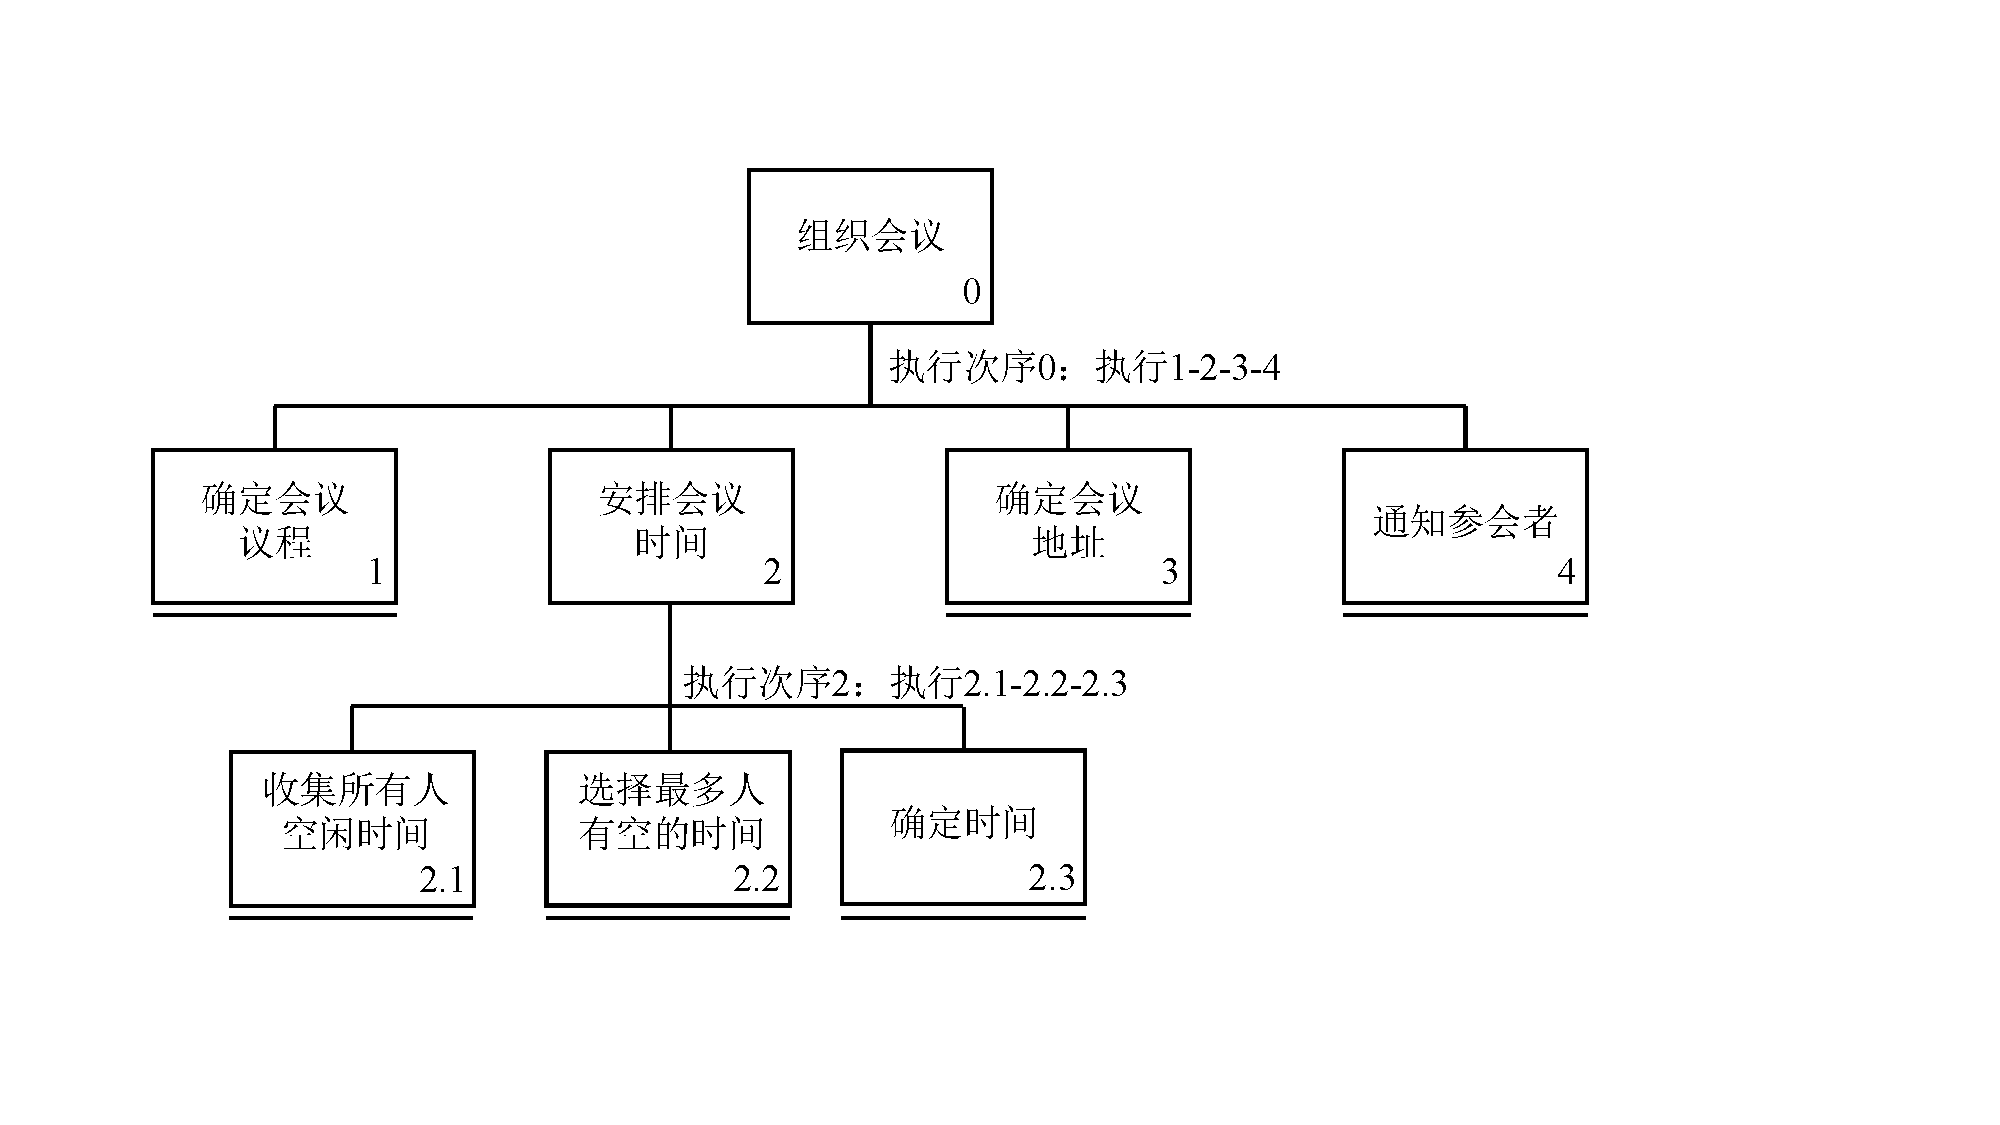
\includegraphics[width=0.63\textwidth]{3.pdf}
    \vspace{-1em}
\end{figure}
\end{solution}



\begin{problem}
为下列每一种情况选择一个适当的评估方法。在每一种情况中确定:
\vspace{-0.8em}
\begin{multicols}{4}
    \begin{enumerate}[label=\arabic*.]
        \item 典型用户
        \item 应用的技术
        \item 代表性的测试任务
        \item 评价标准
    \end{enumerate}
\end{multicols}
\vspace{-1em}
\begin{enumerate}[label=\arabic*.,start=5]
    \item 实验过程(简要描述即可,不需要罗列详细测试步骤)
\end{enumerate}

具体情况包括:
\begin{enumerate}[label=\alph*.]
    \item 你有一个戏院订票系统的原型,潜在的戏迷应用它能减少在售票处前排队。
    \item 你已经设计和实现了一个新的游戏系统,在发布以前你想对其进行评估。
    \item 已经要求你开发一个存储和管理学生考试结果的系统。在实现和给出原型之前,你希望对两个不同的设计进行测试。
\end{enumerate}
\end{problem}

\begin{solution}
\begin{enumerate}[label=\alph*.]
    \item 
    \begin{enumerate}[label=\arabic*.]
        \item 评估方法:用户测试
        \item 典型用户:戏迷
        \item 应用的技术:DECIDE模式
        \item 代表性测试任务:比较新订票系统和原有订票方式的效率
        \item 评价标准:新系统订票所有时间比原有订票方式快15\%为好,10\%-15\%为普通,小于10\%为差
        \item 实验过程:让两组用户分别用新旧两种方式进行订票,记录时间,统计分析
    \end{enumerate}
    \item 
    \begin{enumerate}[label=\arabic*.]
        \item 评估方法:用户测试、用户观察
        \item 典型用户:游戏爱好者
        \item 应用的技术:边说边做、DECIDE模式
        \item 代表性测试任务:新游戏系统的可用性和用户体验情况
        \item 评价标准:对于界面,用户满意度>85\%为优,70\%-85\%普通,70\%以下为差;对于游戏情节设置:响应时间为优
        \item 实验过程:安排用户学习体验游戏系统,可在过程中有道用户说出自己想法,并进行记录。之后发放问卷调查用户体验,统计数据,分析
    \end{enumerate}
    \item 
    \begin{enumerate}[label=\arabic*.]
        \item 评估方法:专家访问
        \item 典型用户:教务人员老师
        \item 应用的技术:问卷调查、访谈
        \item 代表性测试任务:了解用户对于两个设计方案的看法,并进行比较
        \item 评价标准:在不同的方面分别进行比较,用户满意度高的优
        \item 实验过程:安排用户在一个安静的环境中,将两个设计方案向用户描述,听去用户建议,再发放问卷,对不同方面进行调查,统计数据、分析
    \end{enumerate}
\end{enumerate}
\end{solution}




